%---------------------------------------------------------
\section{Justificación}

\noindent
La educación es uno de los factores que más influye en el avance y progreso de personas y sociedades. 
Provee conocimientos, enriquece la cultura, el espíritu, los valores y todo aquello que nos caracteriza 
como seres humanos, pues es la propia educación necesaria en todos los sentidos, por ejemplo, alcanzar 
mayor bienestar social y de crecimiento económico, acceder a mejores niveles de, elevar las condiciones 
culturales, vigorizar los valores cívicos y laicos, para el avance democrático, o bien, para impulsar 
la ciencia, la tecnología y la innovación. \cite{UNAM_Importancia}

\noindent
\newline
Sin embargo, la educación, aunque es pieza clave para un buen desarrollo, es cambiante de región en región.
En Europa, por ejemplo, las políticas o estrategias dependen del nivel educativo, se procura promover la 
educación, la investigación y la innovación; con un enfoque competitivo, favoreciendo la excelencia. 
Para lograr esto, se proveen datos e información actualizada sobre las tareas laborales actuales y 
se le da la oportunidad de desarrollar conocimientos antes de terminar su enseñanza, para que así pueda 
aclarar dudas y aportar ideas. Por otro lado, el sistema educativo latinoamericano no disfruta de una buena 
reputación. En esta región no se le da mucha importancia a la educación, sino que se privilegian otras áreas 
como la economía y la política, sin percatarse de que gran parte de los problemas que afrontan provienen de 
los fallos en la enseñanza. Igual que en Europa, la educación en la región cuenta con los mismos tres niveles,
pero las estadísticas muestran que el número de estudiantes va decreciendo conforme el nivel. \cite{AZ}

\noindent
\newline
Así, en México como en América Latina, la educación -y específicamente la educación superior-, debe persistir
en la búsqueda de una mayor equidad y calidad educativas. Ambos aspectos concentran dificultades y representan 
el mayor reto del sistema en el nivel superior. Las iniciativas deben concentrarse en ampliar las oportunidades 
educativas para más jóvenes, principalmente en las regiones y grupos sociales más 
desfavorecidos, así como en mejorar de forma significativa su oferta educativa. \cite{UNAM_Estado}

\noindent
Por tanto, sabemos que uno de los factores más importantes para el desarrollo es la educación. Sin embargo, 
no siempre se obtienen los resultados más idóneos; ésto se debe a muchas y muy variadas causas que van 
desde la falta de experiencia de los profesores hasta la falta de interés de los alumnos, pasando por el 
poco apoyo de las instituciones para brindar mejores oportunidades de estudio. Mas, una de las causas 
que nos parece de especial relevancia es la falta de atención, dedicación y/o interés de los alumnos a sus 
clases (y tiempos de estudio o extra-clase) y viceversa \cite{UV}. 

\noindent
Por otro lado, las universidades son pocas y de difícil alcance (ya sea por costo o por demanda), tomando 
el peso principalmente la Universidad Nacional Autónoma de México (UNAM) y el Instituto politécnico Nacional 
(IPN). A pesar de ello, y haciendo frente a los problemas, las grandes casas de estudio postulan nuevas ideas 
y alternativas que intenten solventar o atenuar algunos de los problemas que los países y la población tienen 
que enfrentar en materia de educación. 
Creación de planteles, planes de estudio a distancia, nuevas carreras y reestructuración de las actuales son 
estrategias aplicadas por las instituciones mexicanas hoy en día. Por ejemplo, en la Escuela Superior de 
Cómputo (ESCOM) del IPN, en el año 2009 se implementó en cambios del modelo educativo y el rediseño curricular, 
con el objetivo de mantener siempre actualizados los contenidos y las formas de enseñar, para así tener mayores
y mejores resultados de aprendizaje por parte de los estudiantes. 
A pesar de ello, la implementación mencionada que causó desafíos para el desempeño docente, uno de ellos, 
desarrollar competencias pedagógicas. Miguel Zabalza (2003) propuso un esquema de competencias, solo 
describiremos dos \cite{Competencias}.

\begin{itemize}	
	\item Relacionarse constructivamente con los alumnos: Capacidad que se relaciona con la habilidad 
	para entablar relaciones  interpersonales, con la motivación y el liderazgo del profesor, lo que  
	genera climas propicios para el  aprendizaje.
	\item Tutorar: Capacidad de dirigir el proceso de formación integral de nuestros alumnos y que 
	permite acompañarlos a lo largo de su vida escolar.
\end{itemize}

\noindent
El profesor universitario, en esta nueva perspectiva, deja de ser un mero transmisor de conocimientos. La 
formación del estudiante no tiene como único escenario la clase, sino todo el abanico de recursos y espacios 
curriculares: bibliotecas, programas informáticos, portales digitales, actividades diversas en el aula y 
en el entorno, etc. La tutoría académica adquiere también un papel esencial en este nuevo escenario docente. 
\cite{UAB}

\noindent
\newline
A pesar de ello, resulta complicado aplicar estrategias para solventar las deficiencias encontradas en la
educación, pues no solo se trata del sistema o de los profesores, que, aunque influyen en gran manera, no
podemos centrar las soluciones solo en ellos, depende también de la situación académica de los alumnos
y esto a su vez de diversos factores, como la institución a la cual asisten, su situación económica, laboral,
social o familiar. 

\noindent
Así, regresamos a la Escuela Superior de Cómputo, pues creemos que siempre es bueno comenzar desde los 
lugares que nos rodean y en los cuales nos desenvolvemos, bien, nos centramos en la ESCOM, en sus 
estudiantes y en los puntos que Miguel Zabalza menciona. ¿Habrá relación con ellos y con los problemas 
educativos de la ESCOM y México? Para entender mejor la situación de la escuela y poder brindar una propuesta 
de solución, es necesario, como ya explicamos, conocer a la misma, es por ello que nos hemos dado a la tarea 
de involucrarnos más en la comunidad de la ESCOM, en sus problemas y opiniones, preguntando
acerca su vida en la escuela y lo que ésta involucra, dicha encuesta se lleva a cabo con base en la
estadística y lo que ésta establece, con una muestra mínima de 97 personas, según el tamaño de la población
escolar (117 alumnos para este caso). 
A continuación, se muestran algunas de las preguntas realizadas, las respuestas obtenidas y el impacto que
generan para la comunidad de ESCOM. 

\pagebreak
\begin{figure}[htbp!]
	\centering
	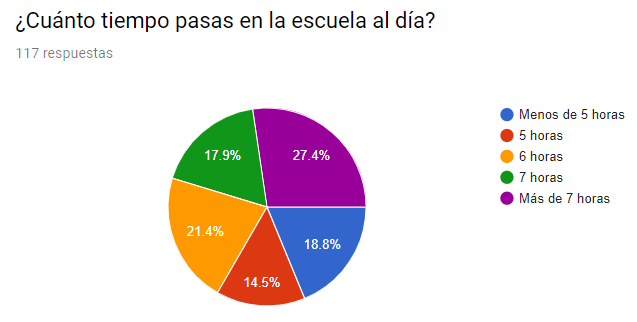
\includegraphics[width=1\textwidth]{intro/images_justificacion/encuesta_horasEnESCOM}
	\caption{Pregunta 1: Sobre el tiempo en la escuela.}
\end{figure}

\begin{figure}[htbp!]
	\centering
	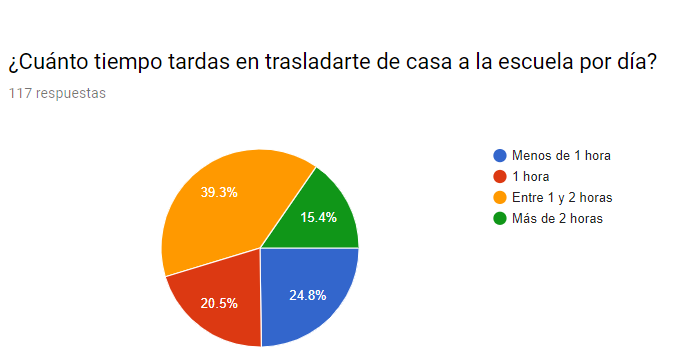
\includegraphics[width=1\textwidth]{intro/images_justificacion/encuesta_horasTraslado}
	\caption{Pregunta 2: Sobre el tiempo en traslado.}
\end{figure}

\pagebreak
\begin{figure}[htbp!]
	\centering
	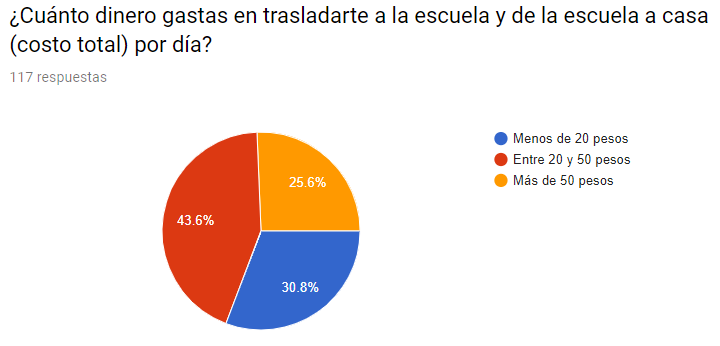
\includegraphics[width=1\textwidth]{intro/images_justificacion/encuesta_dineroTraslado}
	\caption{Pregunta 2: Sobre los recursos en el traslado.}
\end{figure}

\noindent
\newline
Como se puede observar, tenemos un primer acercamiento a la comunidad, y éste nos deja ver dos situaciones
principalmente: el gasto económico que los estudiantes deben realizar para trasladarse de casa a la escuela
y el tiempo que este proceso necesita. Esto resulta especialmente interesante, pues en muchas ocasiones
los muchachos realizan el traslado por cuestiones puntuales como alguna revisión de Trabajo Terminal, alguna
duda sobre una clase específica o bien, para realizar algún proceso académico, obteniendo resultados que
no se esperan, ya que en gran parte de los casos las citas no logran concretarse, debido a que los profesores
se encuentran ocupados o indispuestos, los alumnos no llegaron a tiempo o simplemente se desconoce el lugar y
horario en los cuales los profesores pueden atender el asunto del alumno. \cite{encuesta}. 

\noindent
Esto nos lleva a plantear una solución al problema, accesible para los estudiantes y a la cual puedan
recurrir fácilmente desde cualquier lugar. Con esas premisas, no hay opción distinta a una aplicación móvil,
pues es con ellas que los jóvenes de la actualidad acostumbran a interactuar con el mundo que los rodea, para
nadie es noticia que la tecnología se ha convertido en parte inseparable de la vida social, laboral y 
recreativa de las personas, sobre todo, de las y los jóvenes. \cite{jovenes_tecnologia}. Sin embargo, ¿es una
app móvil realmente del agrado en la comunidad de ESCOM? Y, de ser el caso ¿para qué dispositivos se realizaría?
Bien, para responder a las preguntas anteriores tenemos también las siguientes estadísticas. 

\begin{figure}[htbp!]
	\centering
	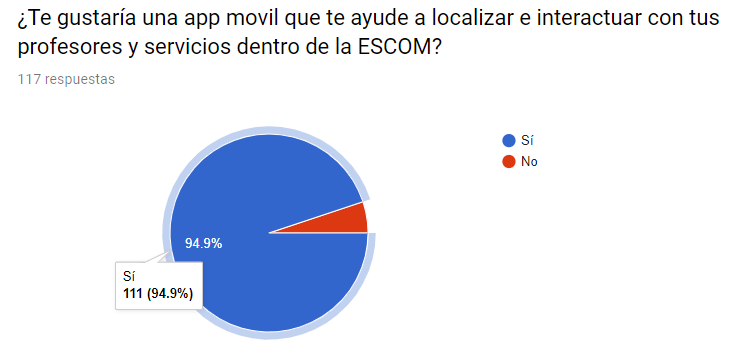
\includegraphics[width=1\textwidth]{intro/images_justificacion/encuesta_agreeApp}
	\caption{Pregunta 4: Sobre la propuesta de una app móvil.}
\end{figure}

\pagebreak
\begin{figure}[htbp!]
	\centering
	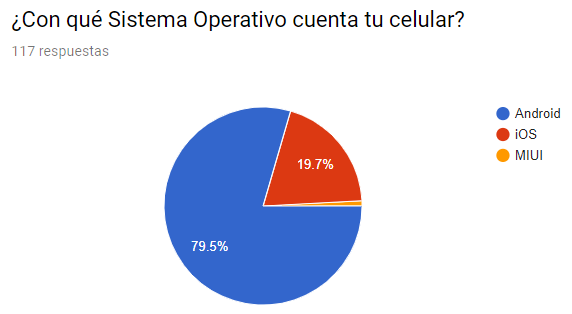
\includegraphics[width=1\textwidth]{intro/images_justificacion/encuesta_so}
	\caption{Pregunta 5: Sobre el sistema operativo más usado.}
\end{figure}

\noindent
\newline
Las preguntas anteriores nos dan pauta a crear la una aplicación, pues a más del noventa por ciento de los
encuestados les gustaría contar con el recurso. Sobre el sistema, el claro ganador es Android, pues casi
el ochenta por ciento de la comunidad cuenta con un teléfono con dicho sistema operativo, si bien lo ideal
sería contar con dos aplicaciones (una por cada sistema operativo), el tiempo nos impide lograr el
desarrollo de éstas, inclinándonos solamente por la app android, pues como ya se mencionó, es el sistema
predominante en ESCOM.

\noindent
\newline
Dicho todo lo anterior, se propone implementar un sistema móvil que ayude a profesores y alumnos a interactuar 
y llevar una mejor comunicación, todo por medio de la difusión de información real acerca de profesores, 
sus horarios, y demás información relevante; así como la posibilidad de generar citas para apoyar el correcto 
aprendizaje de los alumnos o simplemente para atender situaciones académicas que se lleguen a presentar a lo 
largo de los cursos.
Se trata de una aplicación en la cual el usuario (alumnos y profesores) puedan gestionar mejor estos 
tiempos, horarios dedicados al aprendizaje y a la atención de los alumnos. La aplicación se centrará, como 
ya dijimos, en alumnos y profesores, teniendo funcionalidades o perspectivas diferentes para cada uno. Como 
el hecho de generar las citas para los profesores, o la posibilidad que se presenta a los alumnos de 
mantenerse al día con la información relevante y referente a la escuela. Mostrando además un mapa del plantel 
en donde se podrán localizar los diferentes espacios de la escuela, como salones, cubículos o academias. 
Y la posibilidad de buscar a profesores de interés, consultar sus perfiles, horarios y agendar citas, 
mismas que se espera solucionen ciertos problemas que puedan tener los alumnos. Añadiendo, ciertos
puntos de interés para los alumnos, como es consulta de las ofertas de trabajo disponibles para ellos a
través de la bolsa de trabajo. 

\noindent
Así se pretende apoyar a los estudiantes a reforzar su conocimiento y aprendizaje por medio de 
las asesorías y comunicación más cercana con sus profesores, Las competencias anteriores podrán reforzarse
con la ayuda aplicación propuesta que lleva por nombre ESCOMobile.
